\chapter{Zpracování dat}
Vytvořené zařízení inerciální jednotky poskytuje poměrně velké množství dat které je možné různě zpracovávat. Kromě samotných dat z dvou IMU také zaznamenává měřené hodnoty z elektronického kompasu a GNSS modulu. V průběhu vypracování práce se ukázalo, že zpracovat data tak, abychom dosáhli uspokojivých výsledků není vůbec jednoduché a zasloužilo by si samo o sobě rozsah další práce. V této kapitole budou popsány zejména dva postupy zpracování měření, a to výpočet trajektorie čistě z pohybových rovnic a fůze dat s GNSS. Později bylo také zjištěno, že navigace čistě z inerciálních dat nedosahuje uspokojivých výsledků a je zapotřebí korekce dat z GNSS, který ovšem má často ve vnitřních prostorech velmi špatné pokrytí.

Všechny níže popsané skripty byly vytvořené v prostředí MATLAB, jelikož je v něm manipulace s vektory a maticemi jednoduchá. Také můžeme využít již hotových modelů chování senzorů a implementovaných filtrů z Navigation Toolboxu, který je stále poměrně rozsáhle rozšiřován. V elektronické příloze jsou kromě skriptů dostupná i vzorová naměřená data, převedena do formátu csv, které je možné použít k experimentování. Obsahují například chůzi napříč budovou a místností, jízdu autem na venkovním prostranství a měření jednotky v klidu.

\section{Výpočet trajektorie pomocí pohybových rovnic}
Jedná se o základní způsob zpracování dat, který byl popsán v kapitole \ref{INSalg}, které lze nejlépe vystihnout obrázkem  \ref{StrapdownBlock}. Nejdříve je vypočteno z prvního vzorku zrychlení natočení celého zařízení vůči zemi, tedy směr tíhového vektoru. Z tohoto důvodu je potřeba, aby zařízení bylo při začátku měření nepohyblivé. Následně jsou data z gyroskopu integrována numerickou lichoběžníkovou metodou, abychom získali změnu orientace jednotky, ke kterému je přičten výchozí stav.

Z těchto úhlů natočení je vypočtena rotační matice, pomocí které otočíme měřená data zrychlení z body framu do earth framu. Z tohoto rotovaného zrychlení je následně odečten vektor tíhového zrychlení a pomocí dvou dalších numerických integrací otočeného zrychlení vypočteme odhad trajektorie.

Pro demonstraci tohoto postupu byla vytvořena vzorová data chůze ve tvaru obdélníku o rozměrech 3,5 a 4 m. Na začátku a konci těchto měření byla jednotka položena nehybně na stole.

\begin{figure}[h]
     \centering
     \begin{subfigure}[b]{0.49\textwidth}
         \centering
         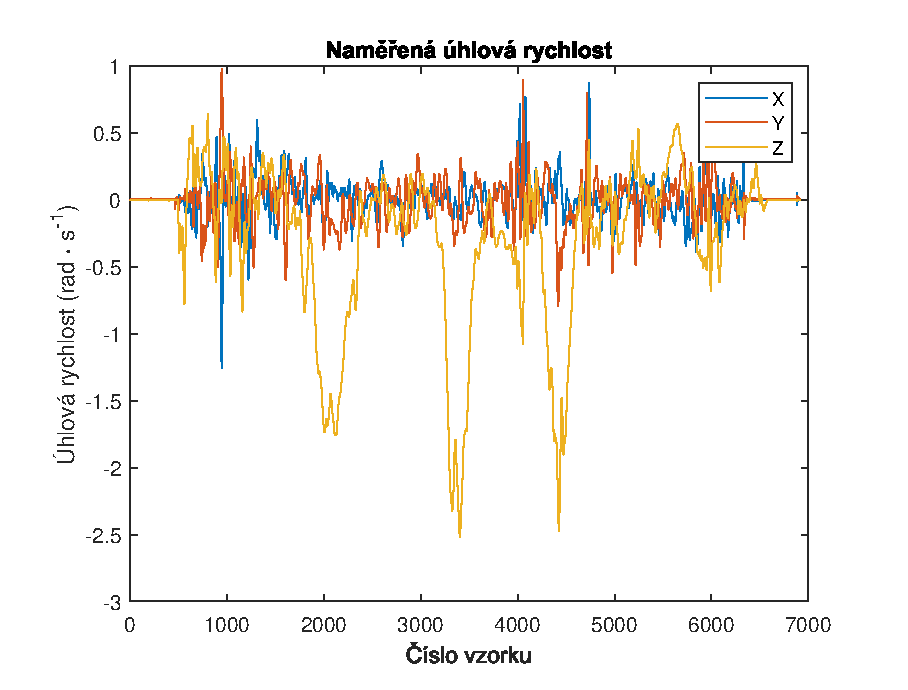
\includegraphics[width=\textwidth]{obrazky/matlab/1measAngularVel}
         \caption{Data z akcelerometru}     
     \end{subfigure}
     \hfill
     \centering
     \begin{subfigure}[b]{0.49\textwidth}
         \centering
         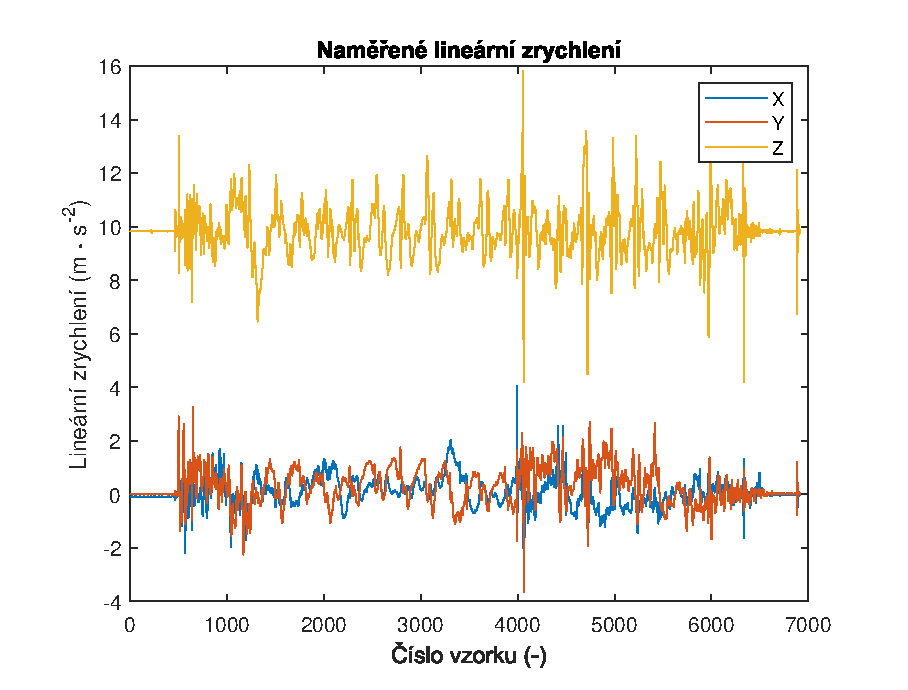
\includegraphics[width=\textwidth]{obrazky/matlab/1measAccel}
         \caption{Data z gyroskopu}   
     \end{subfigure}

        \caption{Záznam dat IMU ADIS16505}
        \label{fig:IMURawData}
\end{figure}

Na obrázku \ref{fig:IMURawData} jsou vidět nezpracovaná zaznamenaná data. Úhlová rychlost v ose Z obsahuje výrazné špičky, jedná se o otáčení v rozích pomyslného čtverce. Na datech akcelerometru je vidět, že celý čas měření byla jednotka převážně ve vodorovné pozici, jelikož lineární zrychlení v ose Z představuje tíhové zrychlení. Zákmity ve zrychlení jsou způsobeny kroky chůze.

\begin{figure}[h]
     \centering
     \begin{subfigure}[b]{0.49\textwidth}
         \centering
         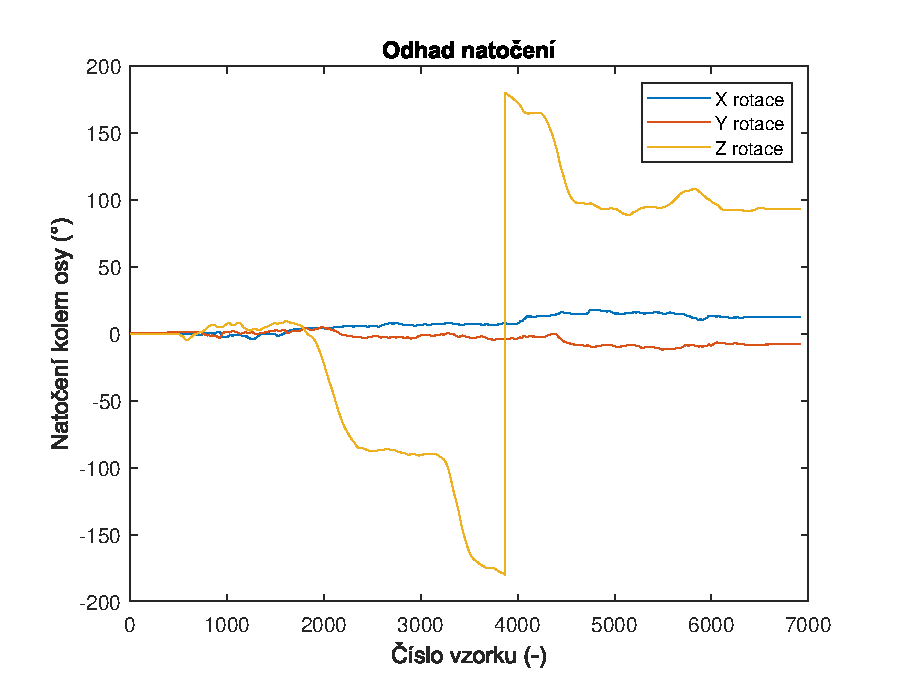
\includegraphics[width=\textwidth]{obrazky/matlab/1measOrient}
         \caption{Natočení jednotky}     
     \end{subfigure}
     \hfill
     \centering
     \begin{subfigure}[b]{0.49\textwidth}
         \centering
         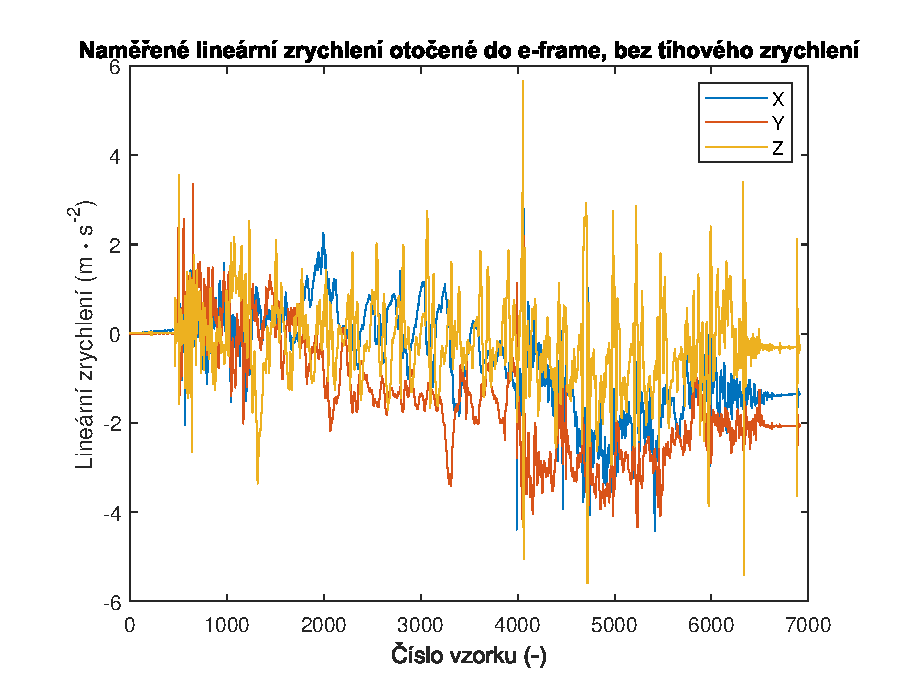
\includegraphics[width=\textwidth]{obrazky/matlab/1measAccelEframeWithoutG}
         \caption{Zrychlení v e-frame bez tíhového zrychlení.}   
     \end{subfigure}

        \caption{Výsledky po první integraci}
        \label{fig:rotationAccel}
\end{figure}

Po integraci dat úhlové rychlosti můžeme určit natočení jednotky a rotovat vektory zrychlení do e-frame. Po odečtení tíhového zrychlení z osy Z dostaneme data na obrázku \ref{fig:rotationAccel}.

